\documentclass[10pt,conference,onecolumn,compsoc]{IEEEtran}

\usepackage{hyperref}
\usepackage{enumitem}
\setlist[itemize]{leftmargin=3 cm}
\setlist[enumerate]{leftmargin=3cm}

\ifCLASSOPTIONcompsoc

 \usepackage[nocompress]{cite}
\else
  % normal IEEE
  \usepackage{cite}
\fi


\ifCLASSINFOpdf
   \usepackage[pdftex]{graphicx}

\else

\fi



\begin{document}
%
\title{2D Top-Down Shooter \\ for UTM CSCI 352 Spring 2017}

\author{Cole Davis and Mel Howard}

\IEEEtitleabstractindextext{%
\begin{abstract}
The proposed game will be a multi-level top-down shooter. The player character will use projectiles to defeat increasing hordes of enemies as he or she progresses through the game. The player progresses by defeating a predetermined number of enemies, allowing them to move to the next location.
\end{abstract}
}


% make the title area
\maketitle


\IEEEdisplaynontitleabstractindextext

\IEEEpeerreviewmaketitle



\section{Introduction}
The game will let users create a Payer and control it vertically and horizontally using the WASD keyboard keys. The Player will travel to different locations, then fight and kill enemies with projectiles from a ranged weapon. This game's target audience is college aged gamers, and retro game enthusiasts. We hope the target audience will at first be engaged, and then extremely frustrated.


\subsection{Background}
A top-down shooter is a game where the user controls his or her character from a birds eye view of their avatar and the surroundings. The proposed game is largely inspired  by \textit{Journey of the Prairie King}, a mini-game in \textit{Stardew Valley}. \textit{Journey} is a top-down where the player's objective is to survive and defeat waves of enemies in stages, all while collecting items the enemies drop. The character creation and starting menus are inspired by the 2D infinite runner, \textit{Magicite}, which randomly generates the player's character and begins game play immediately afterward.

\subsection{Challenges}
One of the most daunting challenges of the proposed game is animating the player avatar and enemies in WPF.
Another issue we anticipate is updating the player score or "kill count" as the Player shoots at enemies.

\section{Scope}
	
	When the proposed game is complete, the user will be able to generate a
character, move it, and shoot projectiles using keyboard controls. The game will have a minimum of six levels that contain a predetermined and increasing numbers of enemies. When the Player shoots an enemy it will ``die,'' and the player's score will be updated.
	
	In the future, we hope to randomly generate levels and enemies, as well as implement an 
item drop system with items that power-up the player character. Another goal we have is to enable return fire from the enemies that cause damage to the Player. 

\subsection{Requirements}
These requirements were gathered based on prior gaming experience.

\subsubsection{Functional}
\begin{itemize}
\item Users will use keyboard controls to move Player around the map
\item Player can shoot enemies with weapon -- only one projectile can be shot at a time
\item Projectiles will either be absorbed by enemies or leave the screen
\item The Player must complete their current  level to advance to subsequent levels
\end{itemize}

\subsubsection{Non-Functional}
\begin{itemize}
\item The (undetermined) minimum frame rate should allow the user to play with suitable performance.
\item The average time between a key press and the event it triggers should be 0.5 seconds and never exceed 2 seconds;
\end{itemize}

\subsection{Use Cases}


\begin{table}
\centering
\begin{tabular}{|c|c|c|c|c|}
\hline
Use Case ID & Use Case Name & Primary Actor & Complexity & Priority \\
\hline 
1 & Move Player & User & Med & \\
\hline
2 & Stop Player & User & Med & \\
\hline 
3 & Shoot & User & Med & \\
\hline

\end{tabular}
\caption{Use Case table}
\label{tab:useCaseIndex}
\end{table}



\begin{itemize}
\item[Use Case Number:] 1
\item[Use Case Name:] Move Player
\item[Description:] A user playing the game wishes to move the Player away from spawning enemies. They will press an arrow key corresponding with the direction to move in. This will trigger the process to move the player. 
\end{itemize}

\begin{enumerate}
\item User decides which direction to move Player
\item User presses arrow key that corresponds with the desired direction
\item Player location is updated as the User holds down the key
\item[Termination Outcome:] The Player is now moving.
\end{enumerate}


\begin{itemize}
\item[Use Case Number:] 2
\item[Use Case Name:] Stop  Player
\item[Description:] A user playing the game is pressing an arrow key to move the Player and releases the key to stop.
\end{itemize}

\begin{enumerate}
\item User decides where to stop the Playe
\item User releases the arrow key
\item Player stops moving
\item[Termination Outcome:] The Player is now halted.
\end{enumerate}


\begin{itemize}
\item[Use Case Number:]3
\item[Use Case Name:] Shoot
\item[Description:] A user is playing a level in the game and enemies begin to spawn. They will press the space bar. This will trigger the process to shoot projectiles.
\end{itemize}
\begin{enumerate}
\item User identifies enemies spawning
\item User moves Player to aim at enemies and presses the space bar
\item Player shoots a projectile at the enemy
\item[Termination Outcome:] The projectile is shot in the direction the Player aimed
\end{enumerate}




\subsection{Interface Mockups}
\begin{figure}[ht!]
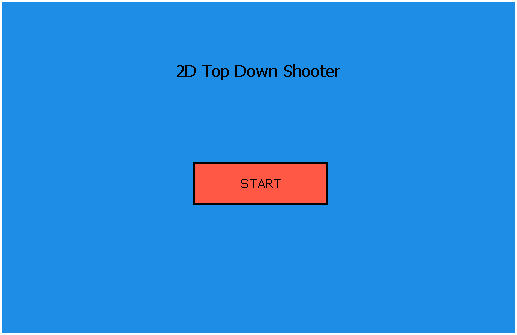
\includegraphics[scale=.25]{Start.png}
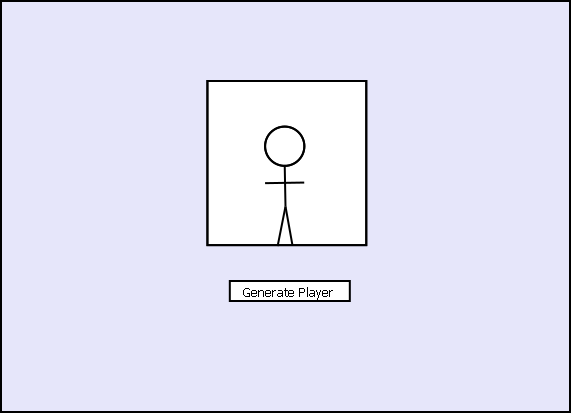
\includegraphics[scale=.25]{Player.png}
\caption{}
\label{UML}
\end{figure}



\section{Project Timeline}
Go back to your notes and look up a typical project development life cycle for the Waterfall approach.  How will you follow this life cycle over the remainder of this semester?  This will usually involve a chart showing your proposed timeline, with specific milestones plotted out.  Make sure you have deliverable dates from the course schedule listed, with a plan to meet them (NOTE: these are generally optimistic deadlines).

\section{Project Structure}
At first, this will be a little empty (it will need to be filled in by the time you turn in your final report).  This is your chance to discuss all of your design decisions (consider this the README's big brother).

\subsection{UML Outline}
Show the full structure of your program.  Make sure to keep on updating this section as your project evolves (you often start out with one plan, but end up modifying things as you move along).  As a note, while Dia fails miserably at generating pdfs (probably my fault), I have had much success with png files.  Make sure to wrap your images in a \texttt{figure} environment, and to reference with the \texttt{ref} command.  For example, see Figure %\ref{cat2}.
\begin{figure}[ht!]
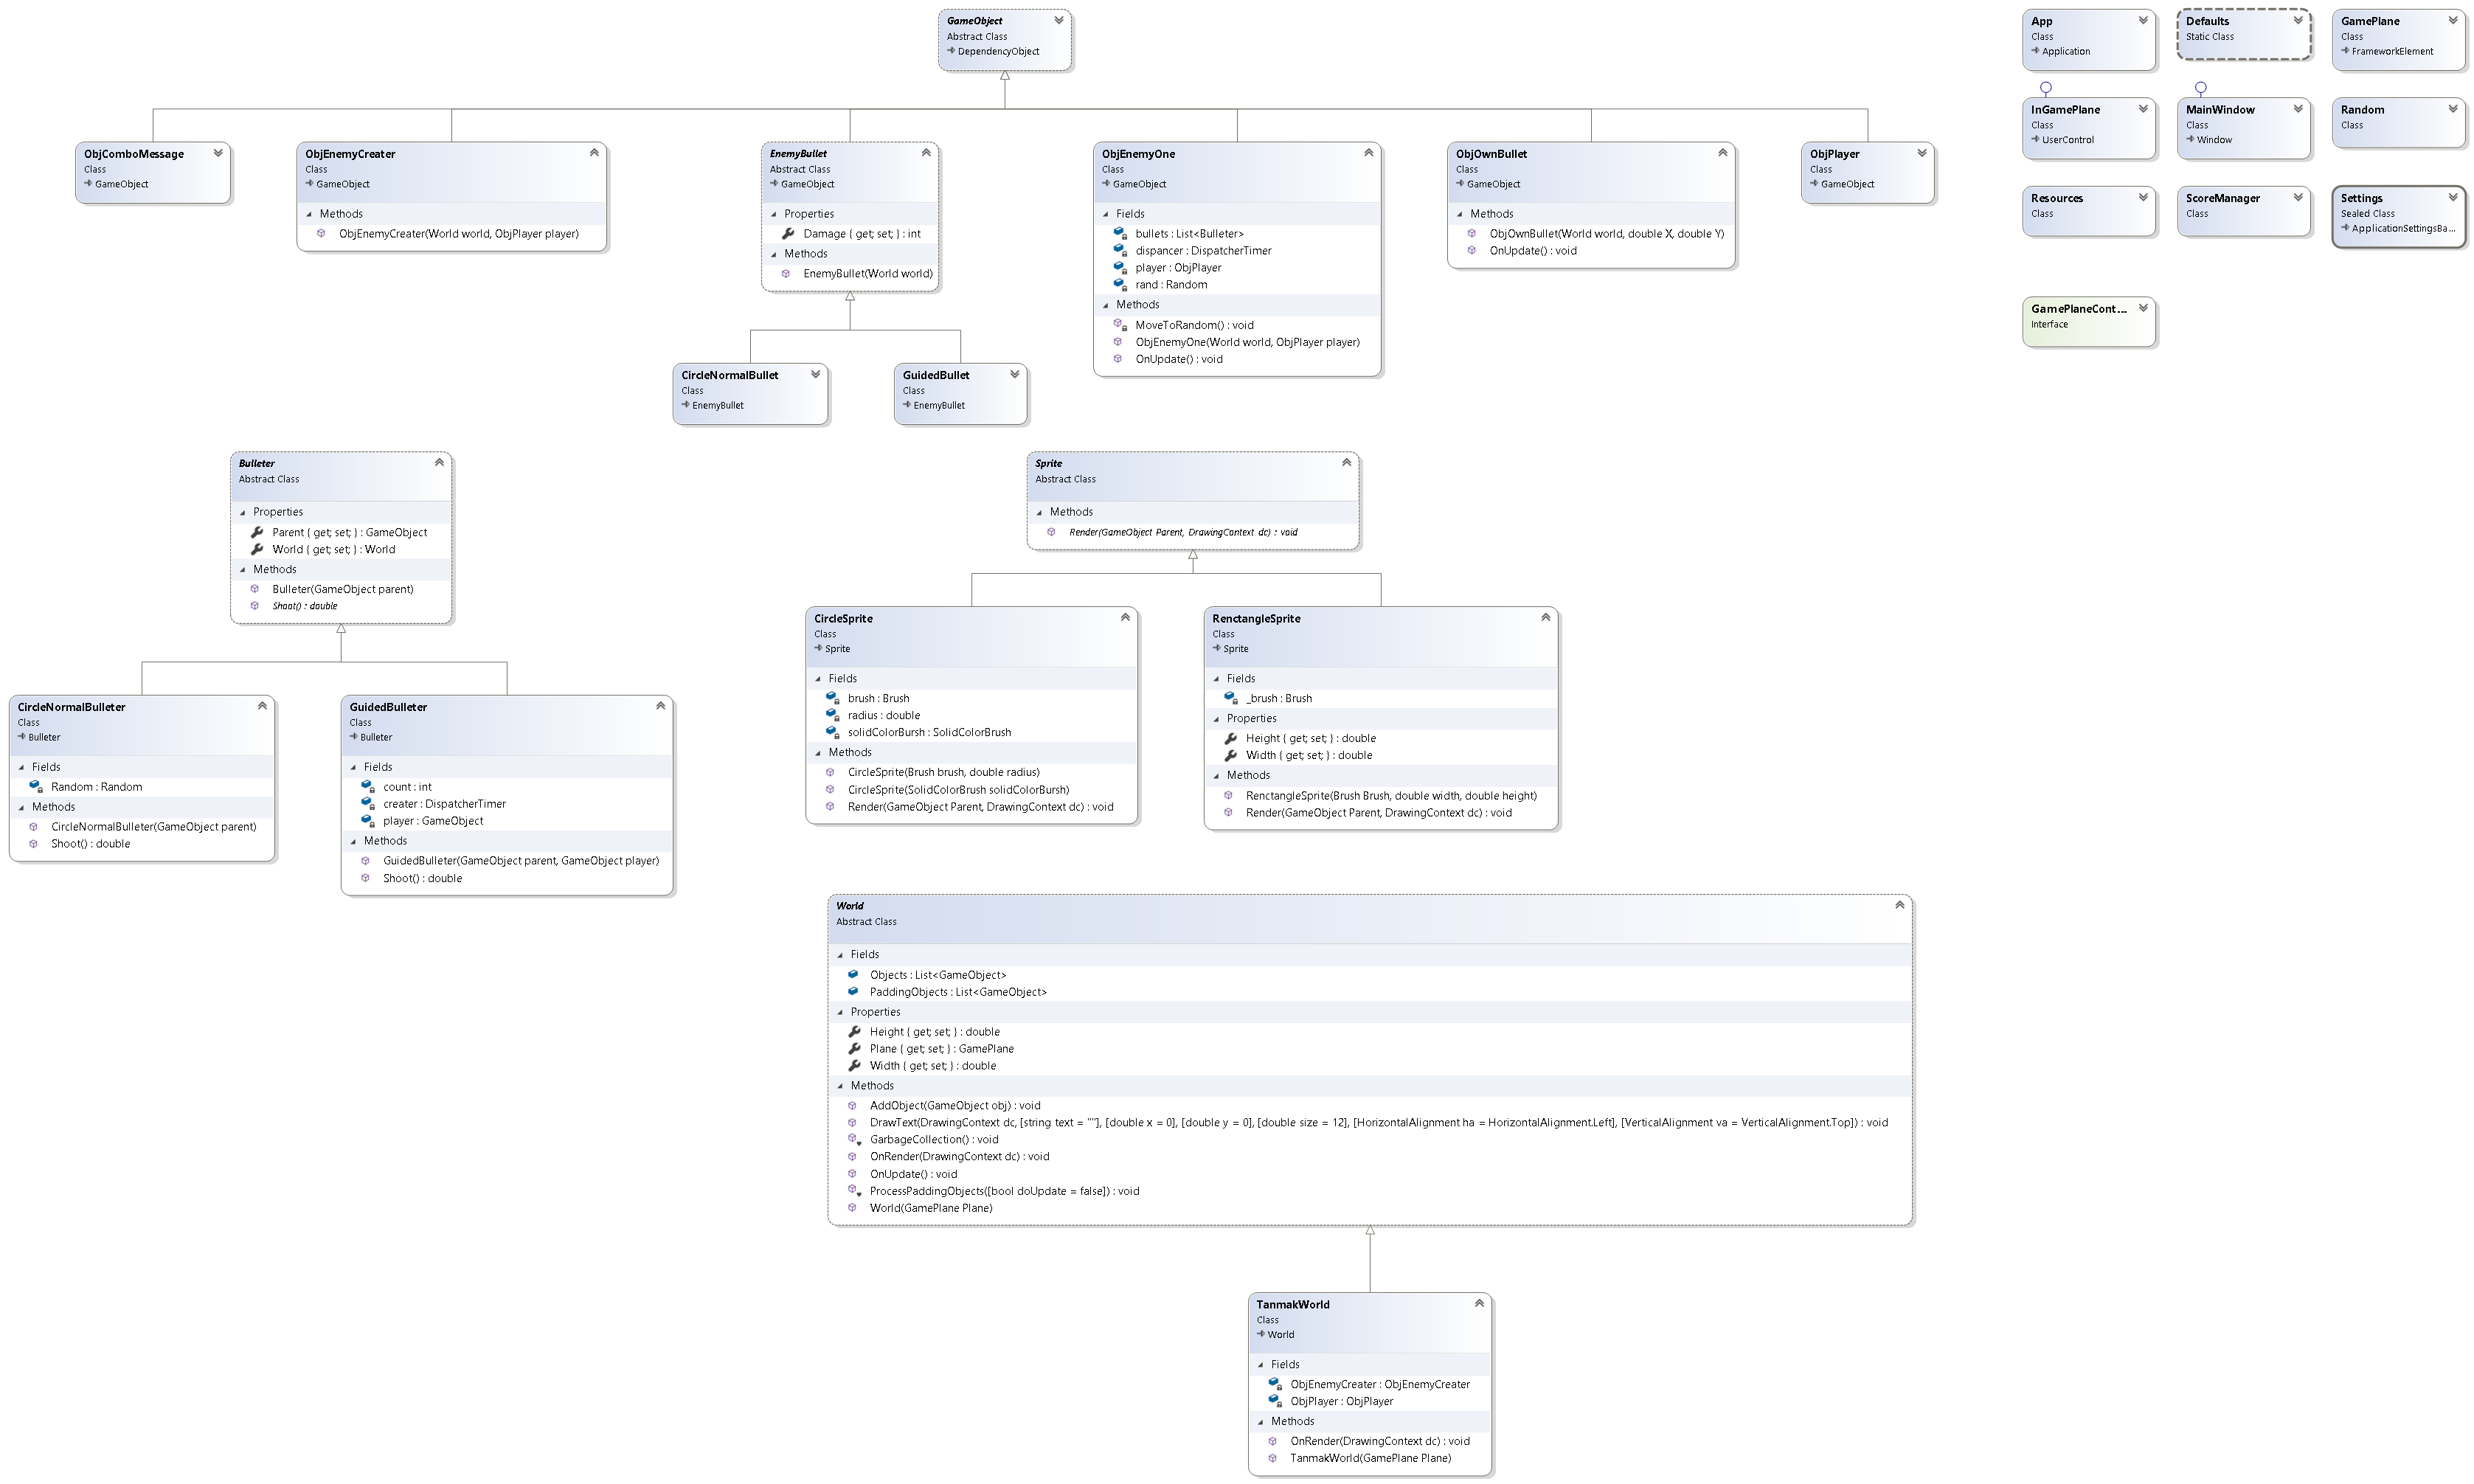
\includegraphics[scale=.25]{ClassDiagram1.png}
\caption{}
\label{UML}
\end{figure}
\begin{figure}[ht!]
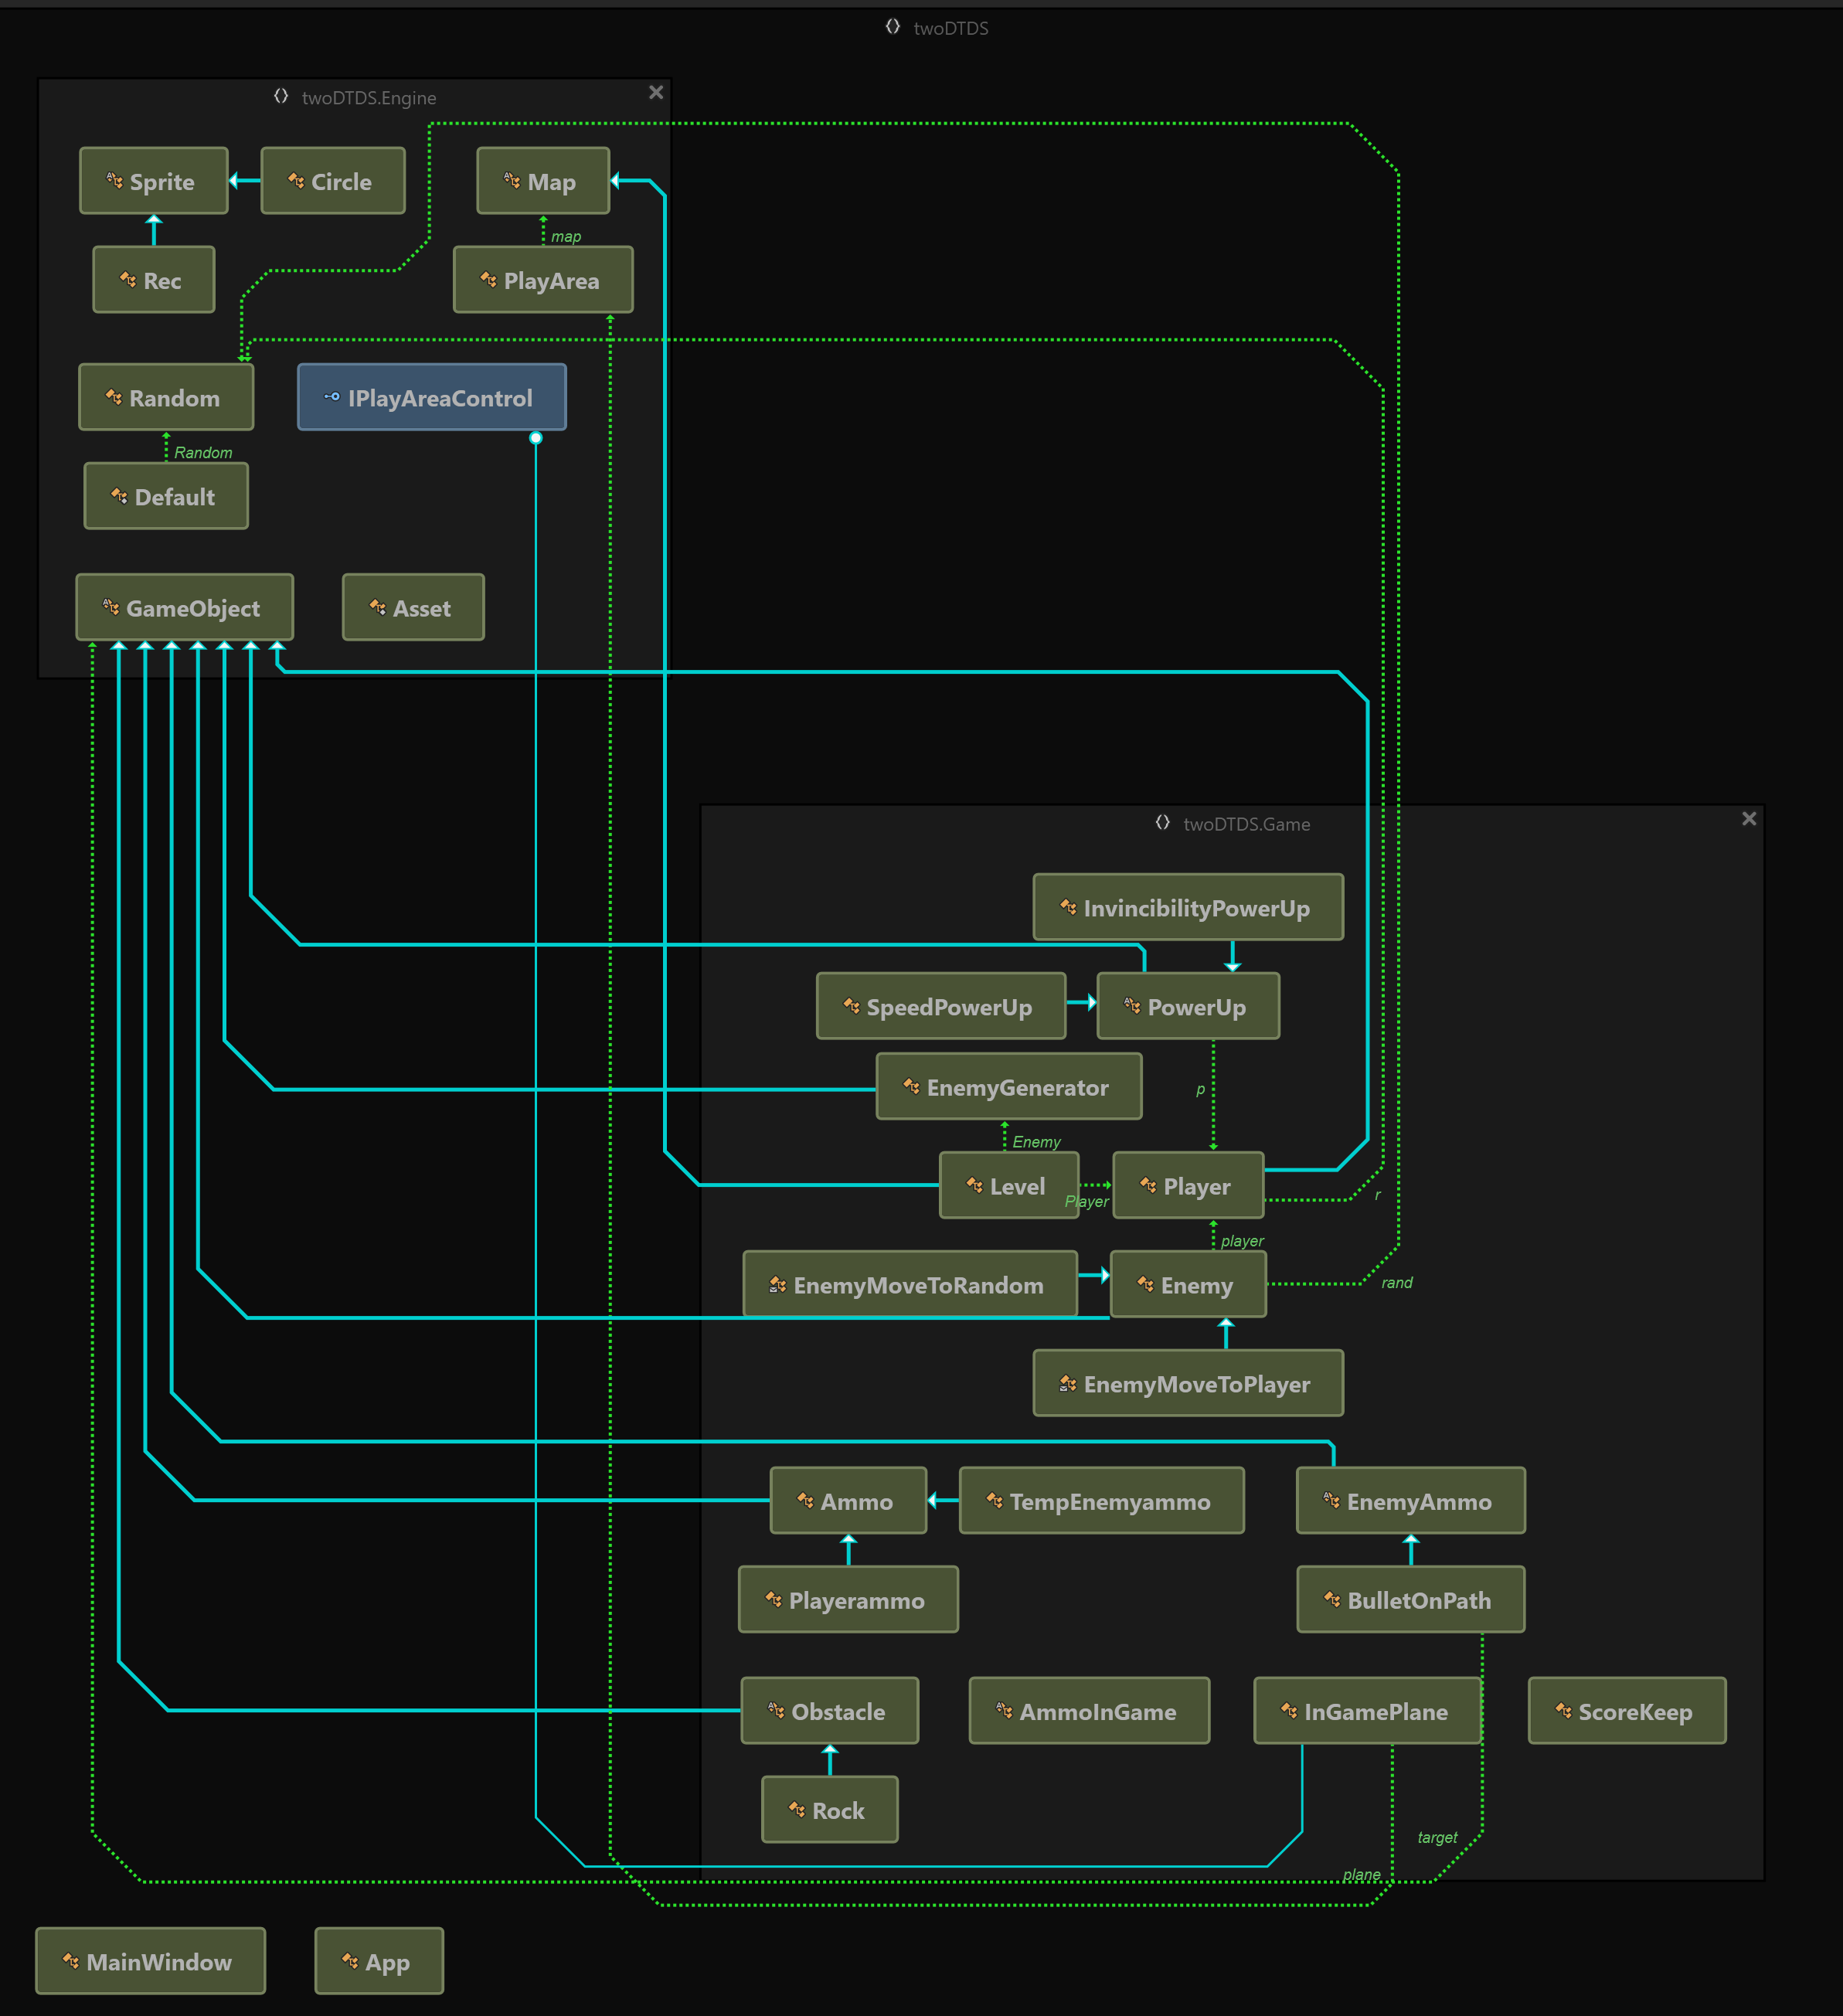
\includegraphics[scale=.25]{Dependencies Graph.png}
\caption{}
\label{UML}
\end{figure}



\subsection{Design Patterns Used}
Make sure to actually use at least 2 design patterns from this class.  This is not normally part of such documentation, but largely just specific to this class -- I want to see you use the patterns!


\section{Results}
\subsubsection*{Deliverable 1:}The team is Mel Howard and Cole Davis. 
The idea so far is to 
have a game of some sort. There are no final concepts.

\subsubsection*{Deliverable 2:}: The idea for the game was decided upon 
to be a 2D Top-Down 
Shooter. We have a fairly solid idea of how we want it to
play and we know our goals. So far, all we have is a square that can move 
around by using the "WASD" keys, which is a decent start.

\subsubsection*{Deliverable 3:} We made some use cases to define some 
definite things that 
we want the user to be able to do, like move with arrow keys
(which we have already acheived), and shoot (not yet acheived). We have 
somewhat of an idea of how the game is going to look. We hope to
implement a menu where you can roll for stats and generates a chracter, and 
then move into the game itself.

\subsubsection*{Deliverable 4:} At this point we have made a huge leap in 
development, with 
a game engine being fully implemented inside its own engine
namespace, along with a few classes created in a game namespace. Some of 
the most important classes we have implemented (if not fully,
almost fully) are an abstract game object, a map/level, a play area, an array 
of various ammo types, a player, and an enemy. You can shoot
bullets, and so can the enemy. No sprites have yet to be added, so right now 
its just windows shapes. There is also no hit detection yet,
and the bullets can only go in one direction.

\subsubsection*{Deliverable 5:} Sprites have been added along with 
backgrounds, but they 
are not yet the final art we hope to use. The player can also now
shoot in multiple directions. There are still no hit boxes, and ammo and 
enemy logic is still to be created. The idea for chracter/stat
generation is most likely dead.

\subsubsection*{Deliverable 6:}A lot has been added by this point. Player 
can now get hit by 
enemy bullets or enimies, there are two enemy types that 
spawn, powerups have a chance at dropping, sprites have been refined, 
enemies can be killed by player shooting at them, you can "roll"
to avoid being hit by enemies, there is a camera shake when player gets hit 
along with invincibility frames, and player can die when
health drops to zero.

\subsection{Future Work}
Where are you going next with your project?
For early deliverables, what are your next steps?  (HINT: you will typically want to look back at your timeline and evaluate: did you meet your expected goals?  Are you ahead of schedule?  Did you decide to shift gears and implement a new feature?)
By the end, what do you plan on doing with this project?  Will you try to sell it?  Set it on fire?  Link to it on your resume and forget it exists?




%\begin{thebibliography}{1}
%
%\bibitem{IEEEhowto:kopka}
%H.~Kopka and P.~W. Daly, \emph{A Guide to \LaTeX}, 3rd~ed.\hskip 1em 
%plus
%  0.5em minus 0.4em\relax Harlow, England: Addison-Wesley, 1999.
%\end{thebibliography}
%
%
%\begin{IEEEbiography}{Michael Shell}
%Biography text here.
%\end{IEEEbiography}
%
%% if you will not have a photo at all:
%\begin{IEEEbiographynophoto}{John Doe}
%Biography text here.
%\end{IEEEbiographynophoto}

% insert where needed to balance the two columns on the last page with
% biographies
%\newpage

%\begin{IEEEbiographynophoto}{Jane Doe}
%Biography text here.
%\end{IEEEbiographynophoto}

% You can push biographies down or up by placing
% a \vfill before or after them. The appropriate
% use of \vfill depends on what kind of text is
% on the last page and whether or not the columns
% are being equalized.

%\vfill

% Can be used to pull up biographies so that the bottom of the last one
% is flush with the other column.
%\enlargethispage{-5in}



% that's all folks
\end{document}


